\documentclass[12pt]{article}

\usepackage[utf8]{inputenc}
\usepackage[T1]{fontenc}
\usepackage[spanish]{babel}
\usepackage{cmbright}
\usepackage{lmodern}
\usepackage{geometry}
\usepackage{pgfplots}
\usepackage{tikz}
\usetikzlibrary{positioning,calc,math,arrows.meta,decorations.markings,intersections}
\usepackage{hyperref}
\usepackage[bf,sf,pagestyles]{titlesec}
\usepackage{titling}
\usepackage[runin]{abstract}
\usepackage[font={footnotesize, sf}, labelfont=bf]{caption} 
\usepackage{siunitx}
\usepackage{graphicx}
\usepackage{booktabs}
\usepackage{amsmath,amssymb}
\usepackage[spanish,sort]{cleveref}
\usepackage{enumitem}

\geometry{
	a4paper,
	right = 2.5cm,
	left = 2.5cm,
	bottom = 3cm,
	top = 3cm
}

\newcommand{\sfbright}{\fontfamily{cmbr}\selectfont}
\renewcommand{\familydefault}{\rmdefault}
\renewcommand{\sfdefault}{cmbr}
\renewcommand{\arraystretch}{1.4}

\hypersetup{
	colorlinks,
	linkcolor = {red!50!blue},
	citecolor = {red!50!blue},
	linktoc = page
}

\numberwithin{table}{section}
\numberwithin{figure}{section}
\numberwithin{equation}{section}

\graphicspath{{./figs/}}

% Unitats
\sisetup{
	inter-unit-product = \ensuremath{ \, },
	allow-number-unit-breaks = true,
	math-celsius = {}^{\circ}\kern-\scriptspace C,
	detect-family = true,
	mode = text,
	list-final-separator = { y },
	list-pair-separator = { y },
	list-units = single,
	separate-uncertainty = true
}

\newcommand{\Z}{\mathbb{Z}}
\newcommand{\N}{\mathbb{N}}
\newcommand{\R}{\mathbb{R}}
\newcommand{\Ry}{\mathit{Ry}}
\newcommand{\conv}[2]{\filldraw[fill = white!50!-red, fill opacity = 0.5, draw = -red!] (#1,0) ellipse [x radius = 0.1, y radius = #2];}
\newcommand{\data}[3]{\SI{#1 \pm #2}{#3}}
\newcommand{\unc}[2]{\ensuremath{{}\pm \SI{#1}{#2}}}
\DeclareMathOperator{\sen}{sen}
\newcommand{\abs}[1]{\left\lvert #1 \right\rvert}
\newcommand{\inn}[2]{\left\langle #1 , #2 \right\rangle}
\newcommand{\parbreak}{
	\begin{center}
		--- $\ast$ ---
	\end{center} 
}
\makeatletter
\newcommand*{\defeq}{\mathrel{\rlap{%
		\raisebox{0.3ex}{$\m@th\cdot$}}%
	\raisebox{-0.3ex}{$\m@th\cdot$}}%
	=
}
\makeatother

\newpagestyle{pagina}{
	\headrule
	\sethead*{\sffamily \bfseries Práctica 4}{}{\theauthor}
	\footrule
	\setfoot*{}{}{\sffamily \thepage}
}
\renewpagestyle{plain}{
	\footrule
	\setfoot*{}{}{\sffamily \thepage}
}
\pagestyle{pagina}

\title{\sffamily {\bfseries Práctica 10:} Efecto fotoeléctrico}
\author{\sffamily B2 2: Arnau Mas, Alejandro Plaza}
\date{\sffamily 6 de junio de 2019}

\begin{document}
\maketitle
\renewcommand{\abstractname}{\sffamily \bfseries Resumen:}
\begin{abstract}
	Se reproduce el efecto fotoeléctrico y se contrastan el modelo clásico ondulatorio y el modelo corpuscular de Einstein, siendo este segundo el único capaz de explicar los fenómenos observados: la intensidad de la luz determina la cantidad de fotones emitidos y su longitud de onda afecta a la energía de cada uno de estos fotones.
	
	Utilizando precisamente el efecto fotoeléctrico se calcula con relativo éxito la constante de Planck gracias a la relación lineal que hay entre la longitud de onda aplicada y el voltaje necesario para detener los electrones arrancados.
\end{abstract}
\hrule

\section{Objetivos}
En esta práctica se pretende estudiar el efecto fotoeléctrico, que consiste en la liberación de electrones ligados a un metal por la acción de una luz incidente. Se evaluará cómo influyen en este proceso la intensidad de la luz, su longitud de onda, etc.

Esta práctica ayudará a entender el comportamiento corpuscular de la luz y los motivos que llevaron a Einstein a proponerlo. Se pretende averiguar si las predicciones del modelo corpuscular de Einstein se ajustan a los datos que se obtengan.

Posteriormente este fenómeno físico será utilizado para estimar la constante de Planck, que es la constante fundamental de toda la física cuántica.

\section{Cuestiones teóricas previas}
El efecto fotoeléctrico se produce cuando se ilumina una placa metálica llamada cátodo y se arrancan electrones que van otra placa llamada ánodo. En el modelo que propuso Einstein la luz está formada por corpúsculos a los que llamó fotones. Cada uno de estos fotones tiene una energía que depende de su frecuencia de oscilación.
\begin{equation}\label{P10Efoton}
	E_{\text{fotón}}=h\nu
\end{equation}
$h$ es la constante de Planck y $\nu$ es la frecuencia.

Cuando un fotón incide sobre el metal, es absorbido enteramente por un electrón que está orbitando en un átomo. Cada electrón absorbe un único fotón de vez. Así cuando un fotón es absorbido por un electrón, toda su energía es transferida al electrón, el cual invierte una parte en trabajo para desligarse del átomo, $q_e\Phi$, y otra se queda en forma de energía cinética $E_c$.
\begin{equation}\label{P10ecuacion}
	h\nu=q_e\Phi+E_c
\end{equation}
Si se quiere extraer un electrón, la mínima energía necesaria para hacerlo es cuando la energía cinética es 0. $h\nu=q_e\Phi$.

Si se quisiese extraer un electrón de un fotocátodo de sodio, cuya función de trabajo es \SI{2.27}{eV}, la frecuencia mínima que habría que aplicarle sería
\begin{equation*}
	\nu_{\text{mín}}=\frac{q_e\Phi}{h}=\frac{ \SI{2.27}{eV} }{ \SI{4.14e-15}{eV s}}= \SI{5.49e14}{Hz},
\end{equation*}
que es aproximadamente la frecuencia del verde.

Al aumentar la frecuencia del fotón, por la ecuación (\ref{P10Efoton}), aumenta su energía y por la ecuación (\ref{P10ecuacion}), ---en el caso en que la energía del fotón es suficiente para arrancar el electrón---, aumenta la energía cinética del electrón, pues la función de trabajo permanece constante. Esto ocurre porque un fotón es absorbido enteramente por un electrón, es decir, la energía del fotón se transmite íntegra a un único electrón, no se divide en varios.

Al aumentar la intensidad manteniendo la frecuencia constante se está incrementando la cantidad de fotones que inciden sobre la placa metálica, pero no la energía de cada uno de estos. Cada electrón absorbe un único fotón, de modo que la energía que tenga el electrón después de absorberlo será independiente de la cantidad de fotones incidentes. Así pues, no variará su energía cinética; lo que variará será la cantidad de electrones extraídos.

Si se pone un voltaje de frenado entre el fotocátodo y el fotoánodo, disminuirá la energía de los electrones. $h\nu=E_c+q_eV+q_e\Phi$. En esta práctica se buscará el voltaje que frene los electrones totalmente, de modo que su energía cinética en en el fotoánodo sea nula.
\begin{equation}\label{P10regresion}
	V=\frac{h}{q_e}\nu-\Phi
\end{equation}
La lámpara con que se ilumina la fotocélula es de corriente alterna, de modo que la intensidad que genera varía periódicamente con el tiempo. Por lo tanto la componente de la señal eléctrica generada por la fotocélula será alterna. No obstante, también se generará una componente continua debida al ruido ambiente (radiación residual que hay en el laboratorio).

El circuito en el que se encuentra la fotocélula hay un amplificador que amplifica únicamente la componente alterna con el fin de minimizar el ruido y observar con mejor precisión la señal de la luz proveniente de la lámpara, que es de la que se pueden controlar parámetros como la frecuencia o la intensidad.

\section{Análisis cualitativo}
Al principio se enciende el osciloscopio y se observa la señal que aparece en su pantalla. Esta es una señal muy débil que corresponde al ruido electromagnético presente en el aire. Cuando se aprietan con los dedos los extremos de los cables a los que se conecta el osciloscopio, se observa un leve incremento de la señal. Esto es debido a que cuando con las puntas del cable se toca un material conductor, la intensidad de la señal se amplifica, pues actúa de antena captando el ruido ambiente. De hecho el cuerpo de un humano es conductor de la electricidad. El efecto se aumenta aún más cuando se toca un objeto metálico, que conduce mejor la electricidad.

Ahora se conecta la lámpara con un filtro de color ---sin importar cuál sea---. La lámpara está conectada a un enchufe, que transmite una corriente alterna de \SI{50}{Hz}, de modo que el voltaje y la intensidad variarán con esa frecuencia. El voltaje $V=V_0\sen\omega t$ y la intensidad $I=I_0\sen\omega t$ están en fase. Esta última se representa en la figura \ref{P10intensidadfilamento}. El filamento de tungsteno se calienta por efecto Joule con una potencia $P=IV=P_0\sen^2\omega t$. Su frecuencia es el doble que la de la intensidad porque el filamento se calienta de igual modo cuando la corriente va en un sentido que cuando va en el otro. Se calienta cuando la intensidad tiene un pico (tanto máximo como mínimo) y se enfría cuando la intensidad es 0. La temperatura varía aproximadamente junto con la potencia y se puede ver en la figura \ref{P10temperatura}.

Por la ley de Stefan-Boltzmann, la potencia que emite un cuerpo ---no necesariamente negro--- es igual al producto de su emisividad, la constante de Stefan-Boltzmann y la cuarta potencia de la temperatura. La intensidad luminosa que llega a la fotocélula es proporcional a la potencia de radiación emitida por la lámpara y viene representada en la figura \ref{P10intensidadluminosa}. Se puede observar que los picos de intensidad máxima son más acusados como consecuencia de elevar a la cuarta. La intensidad eléctrica generada en la fotocélula es proporcional a la cantidad de electrones arrancados del fotocátodo, que a su vez es proporcional a la intensidad luminosa en él incidente. Su dependencia temporal está representada en la figura \ref{P10intensidadfotocelula}.

Como consecuencia de todo esto, la intensidad de corriente eléctrica generada en la fotocélula tendrá forma parecida a una sinusoide con el doble de frecuencia que la corriente eléctrica doméstica, es decir, \SI{100}{Hz}.

\begin{figure}[!ht]
	\begin{center}
		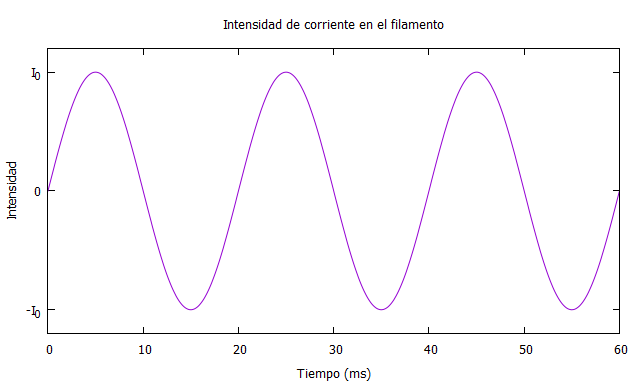
\includegraphics[width=10cm]{P10Intensidadfilamento.png}
		\caption{Esquema de la intensidad de corriente eléctrica que circula por el filamento de la lámpara en función del tiempo.}\label{P10intensidadfilamento}
	\end{center}
\end{figure}
\begin{figure}[!ht]
	\begin{center}
		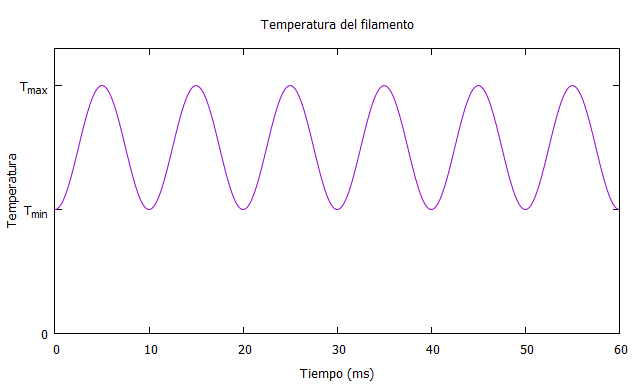
\includegraphics[width=10cm]{P10Temperatura.png}
		\caption{Esquema de la temperatura del filamento de la lámpara en función del tiempo.}\label{P10temperatura}
	\end{center}
\end{figure}
\begin{figure}[!ht]
	\begin{center}
		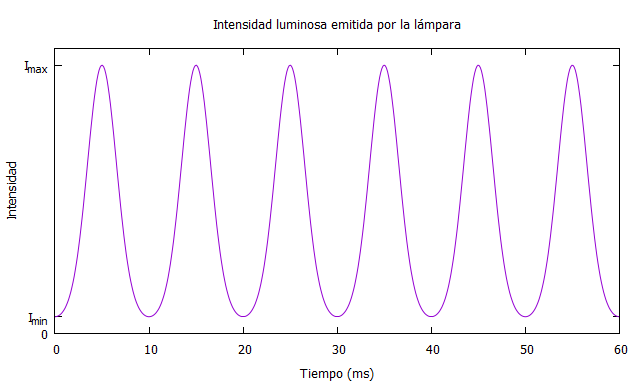
\includegraphics[width=10cm]{P10Intensidadluminosa.png}
		\caption{Esquema de la intensidad luminosa que emite el filamento de la lámpara en función del tiempo.}\label{P10intensidadluminosa}
	\end{center}
\end{figure}
\begin{figure}[!ht]
	\begin{center}
		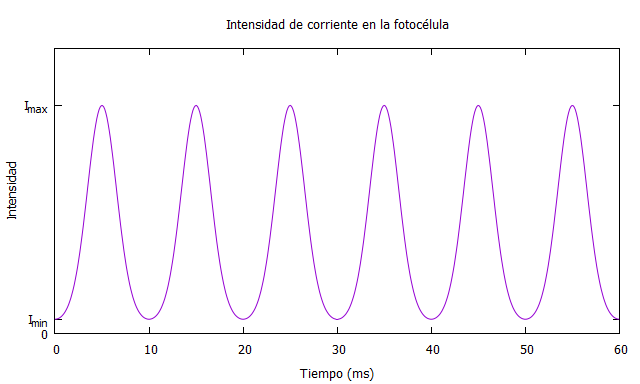
\includegraphics[width=10cm]{P10Intensidadfotocelula.png}
		\caption{Esquema de la intensidad de corriente eléctrica que atraviesa la fotocélula en función del tiempo.}\label{P10intensidadfotocelula}
	\end{center}
\end{figure}

Al medir la señal producida por la fotocélula y que llega al osciloscopio, se observa que es una onda periódica con período \data{10}{1}{ms}. Su frecuencia es la inversa del período y es \data{100}{10}{Hz}, tal como se había predicho. Su incertidumbre ha sido calculada con la expresión (\ref{P10incfreq}) del anexo.

\section{Análisis cuantitativo}
En esta parte de la práctica se mide el voltaje de frenado  necesario para detener los electrones antes de que lleguen al fotoánodo. Para ello se mira con el osciloscopio la señal de la célula fotoeléctrica y se va aumentando el potencial de frenado hasta que la señal del osciloscopio se hace plana. En ese momento el potencial que se está aplicando entre las dos placas es el que aparece en la ecuación (\ref{P10regresion}). Se repite el proceso para varios filtros de diversas frecuencias. Cuanto mayor sea la frecuencia, tanto mayor será la energía de los electrones arrancados y por ende mayor se espera que sea el voltaje de frenado.

Cada filtro tiene toda una curva de transmisión para el espectro electromagnético. Esta curva tiene un pico alrededor de una cierta longitud de onda, pero también transmite otras longitudes, aunque con menos intensidad. Sin embargo a la hora de asignar una longitud de onda a un filtro también se ha de tener en cuenta que el espectro de emisión de la lámpara no es uniforme: es mayor en el centro de la parte visible y menor cerca del ultravioleta y del infrarrojo. En cada filtro se elige una longitud de onda que esté cerca del máximo de transmisión y que la lámpara emita con una intensidad suficiente.

En las gráficas de transmisión en función de la longitud de onda de los filtros, el eje x está dividido en intervalos de \SI{5}{nm}, que se coge como incertidumbre de $\lambda$. La frecuencia se calcula con la expresión $\lambda\nu=c$ y su incertidumbre con la fórmula de propagación de errores.

Al medir el voltaje de frenado, el voltaje que marca la ruleta del aparato que aplica el potencial regulable coincide con el medido con un polímetro, pero en este último se tiene más precisión, de modo que se coge el valor que marca el polímetro.
\begin{figure}[!ht]
	\begin{center}
		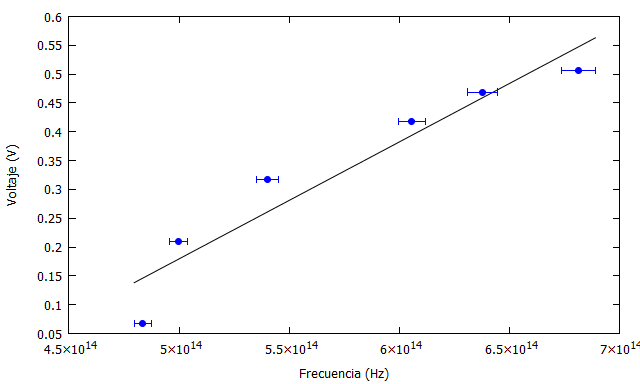
\includegraphics[width=10cm]{P1016,3cm.png}
		\caption{Representación del voltaje entre las placas en función de la frecuencia de la radiación con la lámpara a una altura de \SI{16.3}{cm}. Se incluye la recta de regresión lineal de pendiente \data{2.03}{0.32e-15}{V Hz^{-1}} y de ordenada en el origen \data{-0.83}{0.18}{V}. Sus incertidumbres se han calculado con las fórmulas (\ref{P10incpend}) y (\ref{P10incord}) respectivamente. El coeficiente de correlación es \num{0.910}.}
		\label{P1016,3cm}
	\end{center}
\end{figure}
\begin{figure}[!ht]
	\begin{center}
		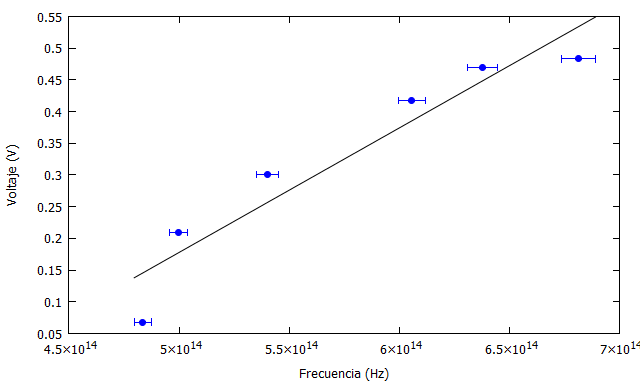
\includegraphics[width=10cm]{P1023,5cm.png}
		\caption{Representación del voltaje entre las placas en función de la frecuencia de la radiación con la lámpara a una altura de \SI{23.5}{cm}. Se incluye la recta de regresión lineal de pendiente \data{1.96}{0.32e-15}{V Hz^{-1}} y de ordenada en el origen \data{-0.80}{0.19}{V}. Sus incertidumbres se han calculado con las fórmulas (\ref{P10incpend}) y (\ref{P10incord}) respectivamente. El coeficiente de correlación es \num{0.903}.}
		\label{P1023,5cm}
	\end{center}
\end{figure}
En las figuras \ref{P1016,3cm} y \ref{P1023,5cm} se ve el voltaje de frenado medido con filtros de distintas frecuencias, así como la recta de regresión a la que ajustan los puntos experimentales. En la primera gráfica la lámpara se encuentra a \SI{16.3}{cm} y en la segunda a \SI{23.5}{cm}. Se observa claramente que los voltajes son muy similares en ambos casos y las rectas de regresión también. Esto es así porque cuando se mueve la lámpara de posición se está variando la intensidad con que la radiación llega a la fotocélula. Cuanto más alejada se encuentra la lámpara, menor es la intensidad con que llega la luz como consecuencia de la atenuación. Sin embargo las frecuencias de la luz al incidir sobre la fotocélula son las mismas, pues dependen de los filtros y se han usado los mismos en ambos casos.

Como se ha explicado anteriormente, si se varía la intensidad pero no la frecuencia de la radiación incidente, se cambia la cantidad de electrones que son arrancados, pero no su energía. El voltaje de frenado depende únicamente de la energía con que salen los electrones, no de la cantidad de estos. Por eso las gráficas son similares; varían únicamente en pequeñas componentes aleatorias al realizar las medidas. De hecho esta independencia de la intensidad se ve de forma matemática en la relación (\ref{P10regresion}), donde no aparece la intensidad.

El coeficiente de correlación lineal es cercano a 1, aunque quizá no demasiado. Además se ve que la recta de regresión lineal no entra dentro de las incertidumbres de los puntos. Esto se debe a que la incertidumbre que se ha cogido es demasiado pequeña. De hecho la incertidumbre del voltaje es más pequeña que el grosor de los puntos y no se ve. Hay todo un rango de voltajes en los que la señal del osciloscopio parece ser 0, de manera que la incertidumbre del voltaje es mayor que únicamente la precisión del polímetro. Además está el ruido que, aunque es disminuido por el amplificador, aún interfiere en la señal y hace que no se mida el valor exacto del voltaje. Por su parte la elección de la longitud de onda es un poco arbitraria: donde parece que coinciden una gran transmisión del filtro con una gran emisión de la lámpara. Sin embargo esta decisión es muy aproximada y a la hora de tomar la incertidumbre se está cogiendo únicamente la longitud de cada división del eje horizontal en las gráficas.

Todo esto genera un cierto error y hace que el coeficiente de correlación no sea tan cercano a 1 como se podría esperar ---aunque sí que se acerca---.

Con la recta de regresión se pueden calcular la función de trabajo del metal del fotocátodo y la constante de Planck. En la ecuación de la recta (\ref{P10regresion}) se ve que la ordenada en el origen es $b=-\Phi=-\frac{q_e\Phi}{q_e}$ donde $q_e\Phi$ es la función de trabajo. También se tiene la pendiente $m=\frac{h}{q_e}$. Se pueden despejar los valores de $h$ y $q_e\Phi$. Sus incertidumbres se calculan con la fórmula de propagación de incertidumbres. El  valor verdadero de la constante de Planck es \SI{6.626e-34}{J s} y el de la carga eléctrica del electrón es \SI{1.602e-19}{C}.

Con la lámpara a \SI{16.3}{cm} se tiene una función de trabajo $q_e\Phi= \data{1.34}{0.30e-19}{J}$ y una constante de Planck $h= \data{3.25}{0.51e-34}{J s}$. Es aproximadamente la mitad del valor verdadero; su discrepancia es del $51\%$.

Con la lámpara a \SI{23.5}{cm} la función de trabajo calculada experimentalmente vale $q_e\Phi= \data{1.29}{0.30e-19}{J}$ y la constante de Planck experimental es \data{3.15}{0.52e-34}{J s} con un discrepancia del $53\%$. Los datos experimentales son bastante dispares con el valor de la constante. Esto es debido a lo comentado anteriormente, sumado a una posible mala calibración del aparato con que se estudia el efecto fotoeléctrico.

Cuando se aumenta la diferencia de potencial entre el fotocátodo y el fotoánodo más allá del voltaje de frenado en el cual los electrones se detienen totalmente, se vuelve a ver una señal sinusoidal como la que se veía sin poner un voltaje de frenado, similar a la de la figura \ref{P10sinusoide}.

Este fenómeno podría ser debido a que los electrones no solo salieran del fotocátodo y llegaran al fotoánodo, sino que también hubiera electrones que viajaran al revés: la luz que incide sobre el fotoánodo arrancase de ahí electrones que fueran a parar al fotocátodo. Para comprobar esta hipótesis se tapará el fotoánodo, de modo que solo haya electrones viajando del cátodo al ánodo. Si los voltajes de frenado varían, entonces quiere decir que sí que hay electrones viajando del ánodo al cátodo.

\begin{figure}[!ht]
	\begin{center}
		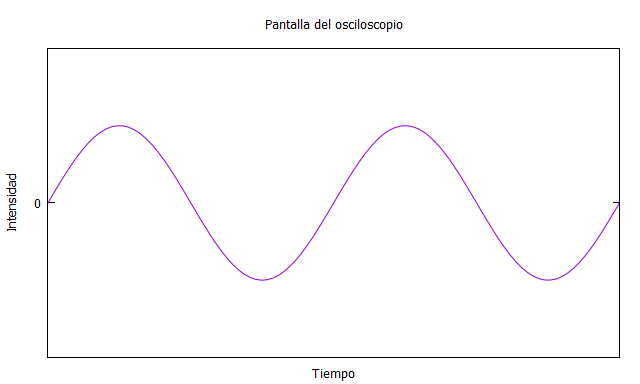
\includegraphics[width=10cm]{P10Sinusoide.png}
		\caption{Esquema de la señal vista en el osciloscopio al aumentar el voltaje más allá del voltaje de frenado.}
		\label{P10sinusoide}
	\end{center}
\end{figure}
\begin{figure}[!ht]
	\begin{center}
		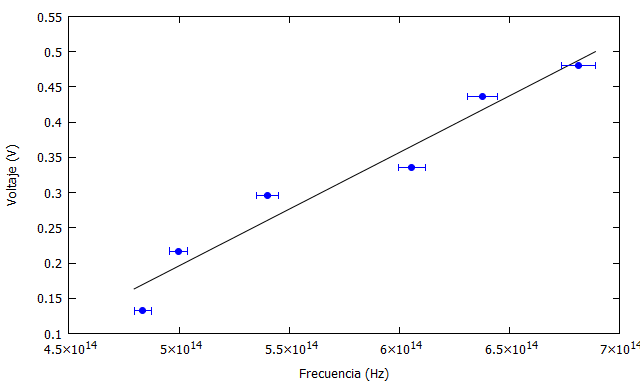
\includegraphics[width=10cm]{P10Anodotapado.png}
		\caption{Representación del voltaje entre las placas en función de la frecuencia de la radiación con el ánodo tapado. Se incluye la recta de regresión lineal de pendiente \data{1.61}{0.19e-15}{V Hz^{-1}} y de ordenada en el origen \data{-0.61}{0.11}{V}. Sus incertidumbres se han calculado con las fórmulas (\ref{P10incpend}) y (\ref{P10incord}) respectivamente. El coeficiente de correlación es \num{0.949}.}
		\label{P10anodotapado}
	\end{center}
\end{figure}

En la figura \ref{P10anodotapado} se ven los voltajes de frenado con el ánodo tapado. Efectivamente son distintos, lo cual indica que antes algunos electrones iban del ánodo al cátodo. En estas nuevas circunstancias el coeficiente de correlación lineal ha ascendido y es muy cercano a $1$, lo cual indica que los puntos se ajustan mejor a una recta y que los resultados experimentales son mejores. Esto es causado por haber eliminado una fuente de error: la señal que generaban los electrones que viajaban del ánodo al cátodo ---los cuales no se han tenido en cuenta al deducir la expresión (\ref{P10ecuacion})---.

La función de trabajo es \data{9.7}{1.7e-20}{J} y la constante de Planck obtenida experimentalmente en este caso es \data{2.58}{0.30e-34}{J s} , con una discrepancia del $61\%$. Estos resultados son sorprendentes porque, a pesar de ajustarse mejor a una recta ---como se esperaba al eliminar el error producido por los electrones que viajan al revés---, la constante de Planck calculada tiene más discrepancia que en el caso anterior.

\section{Conclusiones}
Con esta práctica se ha podido comprobar el carácter corpuscular de la luz. Este se manifiesta cuando la luz es absorbida y emitida por los átomos. Es solo con el modelo corpuscular que se pueden explicar las observaciones realizadas; con el modelo ondulatorio las predicciones son completamente distintas.

La teoría clásica de la luz con un comportamiento ondulatorio es útil para explicar su propagación, pues fenómenos como el de difracción son claramente característicos de una onda. Sin embargo, para entender cómo es absorbida y emitida es necesario considerarla constituida por partículas ---que son llamadas fotones---.

Gracias a este modelo y con las medidas pertinentes se ha conseguido dar una aproximación de la constante de Planck.

Lo que propuso Einstein era rompedor con la física clásica y con todo lo que se creía saber sobre la luz. Y sin embargo se ha comprobado en esta práctica que funciona, lo cual nos dice que es fructífero proponer nuevas ideas revolucionarias para explicar fenómenos hasta el momento inexplicables.
\begin{thebibliography}{1}
\bibitem{P10bibguion} \textsc{Grupo de óptica, departamento de física.} \textit{Guión de la práctica 10}. Universidad Autónoma de Barcelona, 2018.
\end{thebibliography}
\newpage

\appendix
\section{Cálculo de incertidumbres}
Recuérdese la fórmula de propagación de incertidumbres de una función escalar $y=f(x_1,\ldots,x_n)$.
\begin{equation}\label{P10incprop}
u_y^2=\sum_{i=1}^n\left(\frac{\partial f}{\partial x_i}\right)^2u_i^2
\end{equation}

Al final del análisis cualitativo se calcula la frecuencia de una señal a partir del período $\nu=T^{-1}$. Su incertidumbre por tanto es
\begin{equation}\label{P10incfreq}
u_\nu=\frac{1}{T^2}u_T.
\end{equation}

La incertidumbre de la pendiente de una recta de regresión lineal es la siguiente.
\begin{equation}\label{P10incpend}
u_m=S_y\sqrt{\frac{n}{\displaystyle{n\sum_{i=1}^nx_i^2-\left(\sum_{i=1}^nx_i\right)^2}}}
\end{equation}
La incertidumbre de la ordenada en el origen de una recta de regresión lineal es la siguiente.
\begin{equation}\label{P10incord}
u_b=S_y\sqrt{\frac{\displaystyle{\sum_{i=1}^nx_i^2}}{\displaystyle{n\sum_{i=1}^nx_i^2-\left(\sum_{i=1}^nx_i\right)^2}}}
\end{equation}
$S_y$ se define así:
\begin{equation}\label{P10incy}
S_y=\sqrt{\frac{\displaystyle{\sum_{i=1}^n(y_i-mx_i-b)^2}}{n-2}}.
\end{equation}

Al calcular la función de trabajo a partir de la ordenada en el origen y la carga eléctrica del electrón la expresión es $q_e\Phi=-bq_e$. Su incertidumbre se calcula con la fórmula \ref{P10incprop} considerando el valor de $q_e$ como valor verdadero que no tiene incertidumbre.
\begin{equation}\label{P10inctrabajo}
u_{q_e\Phi}=q_eu_b
\end{equation}

La expresión para la constante de Planck es $h=mq_e$. Obramos igual que para la función de trabajo a la hora de calcular la incertidumbre.
\begin{equation}\label{P10incPlanck}
u_h=q_eu_m
\end{equation}
\end{document}
